\documentclass[12px]{article}
\setlength{\parindent}{4em}
\usepackage[margin=2cm]{geometry}
\usepackage{graphicx}
\usepackage{amsmath}
\usepackage{amssymb}
\usepackage{enumerate}
\usepackage{pifont}
\linespread{1.5}

\begin{document}
\begin{center}
    \huge\textbf {Section 2.4 The Precise Definition of a Limit}
\end{center}
\large\begin{enumerate}
    \item Recall: The Intuitive Definition of a Limit\\
    \hspace*{2em}When we see the function "$\lim\limits_{x \to 3}f(x)=5 $", we read it "as when $x$ approaches 3, the limit of $f(x)$ equals to 5". By reading this function, we get to know the intuitive
    definition of this function is when $x$ is close to 3, the value of $f(x)$ will be closer and closer to 5 but note that the final value of $f(x)$ will only be sufficiently close to 5 but not exactly 5.
    \\
    \item The Precise Definition of a Limit (Graphically)\\
    \hspace*{2em}Now, in order to introduce the precise definition of a limit, let’s look at the following graph.
    \begin{center}
        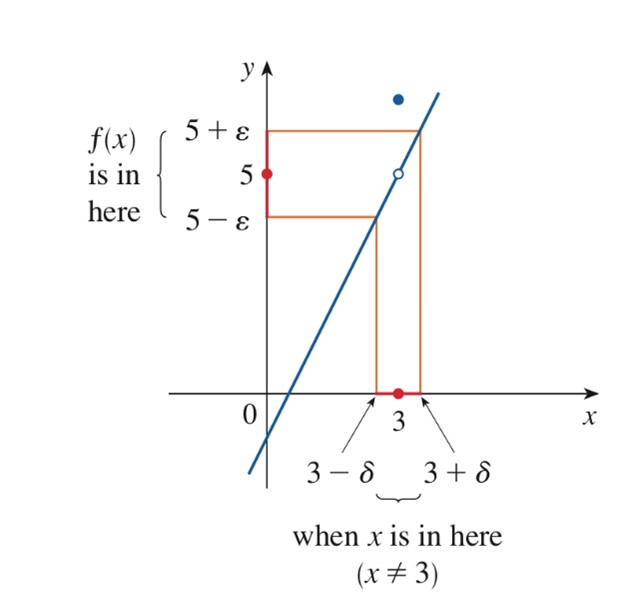
\includegraphics[width=6cm]{pic1.jpg}
    \end{center}
    \hspace*{2em}In the graph, it’s clear to see that when $x$ is in the range of $3\pm\delta$ and approaching 3, $f(x)$ must then be in the range of $5\pm\varepsilon$ and approaching 5. Therefore, we now introduce two new notations, $\delta$ and $\varepsilon$, to explain how close exactly $x$ is regarding to 3 and $f(x)$ is regarding to 5. In the next topic, we’ll be using these two notations to further prove the precise definition of a limit numerically, this proving method is called “the Epsilon-Delta proof”.
    \\
    %3. Epsilon-Delta Definition of Limit (The Epsilon-Delta proof)
    \item Epsilon-Delta Definition of Limit (The Epsilon-Delta proof)\\
    \hspace*{2em} After understanding the graph, we now extend the Epsilon-Delta definition to any limit function, let’s say $\lim\limits_{x \to c}f(x)=L $. In this case, we must discuss two “approaches” on x-axis and y-axis, respectively. \\
    \hspace*{2em}For the approach on y-axis, we can set $y_1$ as the value of $y$, and we can define the distance of $y_1$ and L is $\varepsilon$. ($\left | y_1-L \right | < \varepsilon$) \\
    \hspace*{2em}And the approach on x-axis, we let $x_1$ as the value of $x$, and the distance of $x_1$ and c is defined as $\delta$. ($0 < \left | x_1-c \right | < \delta$)\\
    \hspace*{2em}We can notice the relationship between $\varepsilon$ and $\delta$, “$\varepsilon$ approaching is accomplished by $\delta$ approaching”. To express the relationship with math language:\\
    $$Def.\ "\lim_{x\to\infty} f(x)=L"\ \Leftrightarrow\ \forall\ \varepsilon >0,\ \exists\ \delta>0, $$
    $$s.t.\ \forall\ x\ (\,x\in X\,),\ if\ 0 < \left | x-c \right | < \delta,\ then\  \left | f(x)-L \right | < \varepsilon$$\\
    \item Examples
    \begin{enumerate}[1.]
        %第一題%
        \item Prove $\lim\limits_{x\to1}\ 3x+2=5$\\
        Given $\varepsilon>0, choose\ \delta=$$\underline{\qquad\qquad}>0$\\
        If $0 < \left | x-1 \right | < \delta$\\
        $\Rightarrow\left |(3x+2)-5\right |= \left |\underline{\quad\qquad}\right |=3\left |\underline{\quad\qquad}\right |<\underline{\quad\qquad}$\\
        Since $\varepsilon$ is arbitrary, $\lim\limits_{x\to1}\ 3x+2=5\ (Q.E.D.)$
        \\ 
        %第二題%
        \item Prove $\lim\limits_{x\to2}\ x^2+5=9$\\
        Given $\varepsilon>0, choose\ \delta=min\ (\ 1,\ \underline{\qquad})>0.\quad$\\
        If $0<\left |x-2\right |<\delta$\\
        $\left |x-2\right |<\delta\leq1\Rightarrow\underline{\quad}<x<\underline{\quad}\Rightarrow \underline{\quad}<\underline{\qquad\quad}<\underline{\quad}
        \Rightarrow\left |x+2\right |<5$\\
        $\Rightarrow\left | (x^2+5)-9\right |=\left |x^2-4\right |=\left |\underline{\qquad}\right |\cdot\left |\underline{\qquad}\right |<\left |\underline{\qquad}\right |\cdot\delta<\underline{\qquad}$\\
        Since $\varepsilon$ is arbitrary, $\lim\limits_{x\to2}\ x^2+5=9\ (Q.E.D.)$
        \\
        %第三題%
        \item Prove $\lim\limits_{x\to3}\ \frac{1}{x-1}  = \frac{1}{2}$\\
        Given $\varepsilon>0,\ choose\ \delta=min\ (\ 1,\ \underline{\quad})>0$\\
        If $0<\left |x-3\right |<\delta$\\
        $\left | x-3 \right |<\delta\leq1\Rightarrow\underline{\quad}<x<\underline{\quad}\Rightarrow\underline{\quad}<x-1<\underline{\quad}\Rightarrow\underline{\quad}<\frac{1}{x-1}<\underline{\quad}$\\
        $\Rightarrow\left |\frac{1}{x-1}-\frac{1}{2}\right |=\frac{\left | \qquad\right |}{\ \,\left |\quad\ \right |}=\frac{\left |\quad\ \right |}{\ \,\left |\quad\ \right |}<\frac{\ \ }{\ \,\left |\quad\ \right |}\cdot\delta<\frac{\quad}{\quad}\cdot\delta\leq\frac{1}{2}\cdot2\varepsilon=\varepsilon$\\
        Since $\varepsilon$ is arbitrary, $\lim\limits_{x\to3}\frac{1}
        {x-1}=\frac{1}{2}\ (Q.E.D)$
        \\
        \\
    \end{enumerate}
    \item Exercises
    \begin{enumerate}[1.]
        \item Prove $\lim\limits_{x\to-2}\ (-2x+1)=5$\\
        \\
        \\
        \\
        \\
        \\
        \\
        \item Prove $\lim\limits_{x\to-2}\ (x^2-1)=3$\\
        \\
        \\
        \\
        \\
        \\
        \\
        \item Prove $\lim\limits_{x\to2}\ \frac{1}{x}=\frac{1}{2}$
        \\
        \\
        \\
        \\
        \\
        \\
    \end{enumerate}
\end{enumerate}







\end{document}